 \documentclass[12pt]{article}
\usepackage[a4paper, margin=.30in]{geometry}

\usepackage{array}
\usepackage{graphicx, subfig, wrapfig, fancyhdr, lastpage,makecell }
\newcommand\headerMe[2]{\noindent{}#1\hfill#2}
\usepackage[mathscr]{euscript}



\pagestyle{fancy}
\fancyhf{}

\rfoot{\em{Page \thepage \hspace{1pt} / \pageref{LastPage}}}
\begin{document}

\headerMe{Royaume du Maroc}{année scolaire \emph{2022-2023}}\\
\headerMe{Ministère de l'Éducation nationale, }{  Professeur :\emph{Zakaria Haouzan}}\\
\headerMe{du Préscolaire et des Sports}{Établissement : \emph{Lycée SKHOR qualifiant}}\\

\begin{center}

    \vspace{-1.5cm}
Devoir  N°2 \\
   Filière Tronc Commun Scientifique\\
Durée 2h00
\\
\hrulefill
\Large{Chimie 7pts - 36min}
\hrulefill\\

    %\emph{Les Trois parties sont indépendantes}
\end{center}
%end Headerss------------------------
 
    \vspace{-1.2cm}
    
\section*{Le modèle de l'atome  \dotfill (7pts) }
%\begin{wrapfigure}[5]{r}{0.36\textwidth}
    %\vspace{-1.8cm}
    %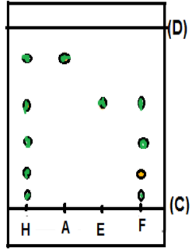
\includegraphics[width=0.36\textwidth]{./img/CCM.png}
%\end{wrapfigure}
L’atome de sodium Na contient 23 nucléons et 11
électrons.

Données : $m_p = m_n = 1,7.10^{-27}kg$ , $1pm = 10^{-12}m$ , $1m^3  =10^6 cm^3$

\begin{enumerate}

\item Déterminer le numéro atomique de cet
atome.\dotfill(1pt)
\item  Donner le symbole de cet atome.\dotfill(1pt)
\item  Calculer la masse de cet atome.\dotfill(1pt)
\item Calculer le nombre des atomes de sodium
contenus dans un échantillon de sodium
de masse $m=23,20g$.\dotfill(2pts)
\item  Le rayon de l’atome de sodium est
$r=190pm$, calculer son volume exprimé en $m^3$ et $cm^3$.\dotfill(1pt)
\item  Donner la formule électronique de cet
atome .la couche externe est-elle saturée
justifier votre réponse.\dotfill(1pt)
\end{enumerate}
%__________________Chimie ______________________-
%%%%%%%+_+_+_+_+_+_+_+_+_Partie1

%_____________________________________PHYSIque Partie 22222____________________________________________________________________________
\begin{center}
    %\vspace{2cm}
\hrulefill
\Large{Physique 13pts - 84min}
\hrulefill\\
    \emph{Les  parties sont indépendantes}
\end{center}
%end Headerss------------------------
\section*{Exercice 1 : Le mouvement \dotfill(8pts)- 48 min }
\vspace{-0.5cm}
 \section*{Partie 1 :Le Mouvement rectiligne uniforme \dotfill(3 pts)}
 On considère deux voitures A et B en mouvement rectiligne uniforme sur une partie d’une autoroute avec les vitesses respectivement $V_A=72Km.h^{-1}$ et $V_B=108Km.h^{-1}$.
%\begin{wrapfigure}{r}{0.36\textwidth}
	\vspace{-0.4cm}
 \begin{center}
	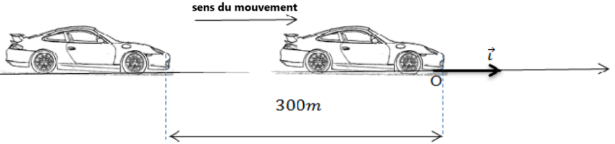
\includegraphics[width=0.56\textwidth]{./img/ex1.png}
\end{center}
%\end{wrapfigure}


	\vspace{-0.4cm}
A l’instant $t=0$ la voiture B est à $300m$ derrière la voiture A.
On choisit la position O, la position de la voiture A à l’instant $t=0$ ; comme origine des abscisses et des dates.

\begin{enumerate}
	\item  Convertir la valeur de $V_A$ et $V_B$ en $m.s^{-1}$.\dotfill(1pt)
	\item Ecrire l’équation horaire du mouvement de chacune des voitures (A) et (B) sur l’axe $(Ox)$.\dotfill(1pt)
	\item  Déterminer l’instant $t$ et l’abscisse $x$ du doublage de la voiture (A) par la voiture (B).\dotfill(1pt)
\end{enumerate}

\section*{Partie 2 : Le Mouvement de l'autoporteur \dotfill(5 pts)}
Un mobile autoporteur S, de masse m, glisse sur un plan horizontal.

On enregistre les positions occupées par un point A du mobile à intervalle de temps $\tau = 40 ms$. On obtient l’enregistrement suivant : 
 \begin{center}
	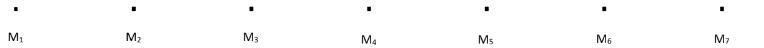
\includegraphics[width=0.8\textwidth]{./img/ex2.png}
\end{center}

\begin{enumerate}

	\item Calculer la vitesse instantanée $V_2$ et $V_4$ respectivement en $M_2$ et $M_4$.\dotfill(1pt)
	\item Déterminer la nature du mouvement du mobile, justifier.\dotfill(1pt)
	\item Représentez $V_2$ en utilisant l'échelle de votre choix.\dotfill(1pt)
	\item On considère $M_2$ l’origine des abscisses et $M_1$ l’origine des dates, déterminer l’équation horaire du mouvement.\dotfill(1pt)
	\item Calculer la distance parcourus par l’autoporteur (S) durant 3s.\dotfill(1pt)
\end{enumerate}


\section*{Exercice 2 : Principe d’inertie \dotfill(5pts) - 36 min }
\section*{Partie 1 : Vérification du concept d'inertie. \dotfill(2,5pts)}

\begin{wrapfigure}[4]{r}{0.36\textwidth}
	\vspace{-0.8cm}
	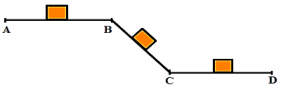
\includegraphics[width=0.36\textwidth]{./img/last.png}
\end{wrapfigure}


Un corps (S) se déplace sur un rail composé de 3 parties. On
lance ce corps du point A avec une vitesse $V_A=1m/s$ , et arrive au point D avec une vitesse $V_D=2m/s$. 

On considère que le contact se fait sans frottement.

\begin{enumerate}
	\item Faire l’inventaire des forces appliquées sur le corps (S), et représenter ces forces sur la figure pour
chaque partie. \dotfill(1pt)
\item Déterminer la partie où le principe d’inertie n’est pas vérifié.\dotfill(0,5pt)
\item Quelle est la valeur de la vitesse du corps (S) au point B, et au point C ? justifier votre réponse.\dotfill(1pt)
\end{enumerate}

\section*{Partie 2 : Le centre d'inertie. \dotfill(2,5pts)}

\begin{wrapfigure}[4]{r}{0.36\textwidth}
	\vspace{-0.8cm}
	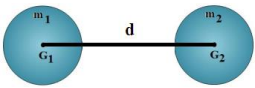
\includegraphics[width=0.36\textwidth]{./img/ex3.png}
\end{wrapfigure}


Deux sphères (A) et (B) de masses respectives $m_1$=$1kg$ et $m_2$=$3kg$ et de centres d’inertie respectives $G_1$ et $G_2$ qui sont séparés par la distance $d = 40 cm$. Ces deux sphères sont liées rigidement et constitue un système comme l’indique la figure ci-contre.

\begin{enumerate}

\item Rappeler la relation barycentrique.\dotfill(0,5pt)
\item Déterminer le centre d’inertie G de ce solide.\dotfill(1pt)
\item Une plaque homogène et d’épaisseur constante, et formée d’une partie carrée et de côté $a=4cm$, et d’une partie triangulaire équilatérale.

	Sachant que \textbf{la masse} de la partie triangulaire est \textbf{3 fois plus légère} que la masse de la partie carrée.

	déterminer la position du centre de masse de la plaque homogène par application d’une méthode de votre choix.\dotfill(1pt)
\end{enumerate}

 \begin{center}
	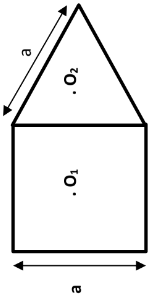
\includegraphics[width=0.16\textwidth]{./img/ex4.png}
\end{center}



\end{document}
